\documentclass[10pt,a4paper]{article}
\usepackage[utf8]{inputenc}
\usepackage[T1]{fontenc}
\usepackage{polski}
\usepackage{lmodern}
\usepackage[a4paper,margin=2.0cm]{geometry}
\usepackage{amsmath,amssymb}
\usepackage{graphicx}
\usepackage{booktabs,tabularx}
\usepackage{caption}
\usepackage{microtype}
\usepackage{xcolor}
\usepackage[colorlinks=true,linkcolor=blue]{hyperref}
\emergencystretch=2em
\captionsetup{font=small,labelfont=bf}
\setlength{\parskip}{3pt}
\setlength{\parindent}{0pt}
% generated by ceiling.py
\newcommand{\CKCStabMedian}{57}
\newcommand{\CKCmax}{185}
\newcommand{\CKCmaxBounded}{185}
\newcommand{\CKCminUnb}{nan}
\newcommand{\CKCminUnbR}{17}
\newcommand{\CKmax}{2.07}
\newcommand{\CKzero}{1.76}
\newcommand{\CSKexp}{2.95}
\newcommand{\CSKlocalReport}{3.47}
\newcommand{\CSKspline}{3.57}
\newcommand{\CSKsplineErr}{0.13}
\newcommand{\CSKsplineHi}{3.69}
\newcommand{\CSKsplineLo}{3.45}
\newcommand{\CcFortyExp}{+3.7}
\newcommand{\CcFortySpl}{+4.3}
\newcommand{\CceilKCmed}{262}
\newcommand{\CceilMaxLong}{11.50}
\newcommand{\CceilMedAll}{10.50}
\newcommand{\CceilMedLong}{10.50}
\newcommand{\CceilMinLong}{8.75}
\newcommand{\CcorrResVefFixed}{+0.46}
\newcommand{\CcorrResVefFree}{+0.37}
\newcommand{\CdChiSixFreeD}{393}
\newcommand{\CdChiSixFreeO}{369}
\newcommand{\CdChiSixFreeT}{385}
\newcommand{\Cfraccexp}{20}
\newcommand{\Cfraccspl}{22}
\newcommand{\CfraccsplUnc}{1}
\newcommand{\Cfraceexp}{-36}
\newcommand{\Cfracespl}{-37}
\newcommand{\ChiOverKMedBounded}{0.20}
\newcommand{\CloNinetyFiveMedStab}{9.65}
\newcommand{\CloRMedStabLong}{9.75}
\newcommand{\ClogKStabErrMed}{0.10}
\newcommand{\ClogKStabMean}{9.82}
\newcommand{\ClogKStabSD}{0.23}
\newcommand{\ClogKbestRMedStabLong}{9.95}
\newcommand{\CmND}{-0.325}
\newcommand{\CmNDErr}{0.020}
\newcommand{\CmNO}{-0.289}
\newcommand{\CmNOErr}{0.020}
\newcommand{\CmNT}{-0.334}
\newcommand{\CmNTErr}{0.021}
\newcommand{\CnAboveCeil}{1}
\newcommand{\CnAboveCeilStabLong}{1}
\newcommand{\CnAll}{104}
\newcommand{\CnBoundedStab}{77}
\newcommand{\CnCensPts}{3}
\newcommand{\CnKCtwenty}{68}
\newcommand{\CnKCtwentyP}{68}
\newcommand{\CnLoUnb}{0}
\newcommand{\CnNotGlobal}{0}
\newcommand{\CnRep}{8}
\newcommand{\CnSim}{14144}
\newcommand{\CnStabAll}{77}
\newcommand{\CnStabLong}{59}
\newcommand{\CnStabLongKC}{55}
\newcommand{\CnStabLongP}{59}
\newcommand{\CnTitr}{108}
\newcommand{\CnUpUnb}{0}
\newcommand{\CnUpUnbKCtwenty}{0}
\newcommand{\CnUpUnbR}{3}
\newcommand{\CnUpUnbRDestab}{0}
\newcommand{\CnUpUnbRKCtwenty}{2}
\newcommand{\CnUpUnbRStab}{3}
\newcommand{\CnUpUnbRStabLong}{3}
\newcommand{\CnUpUnbStabLong}{0}
\newcommand{\CprhoN}{0.04}
\newcommand{\CprhoShiftVef}{0.006}
\newcommand{\CprhoWt}{0.00}
\newcommand{\CrepBroSixSone}{-0.260}
\newcommand{\CrepBroSixStwo}{+0.185}
\newcommand{\CrepBroStwo}{+nan}
\newcommand{\CrepEKnowles}{-0.319}
\newcommand{\CrepFracMeanc}{19.8}
\newcommand{\CrepFracMeane}{-36.3}
\newcommand{\CrepNullE}{-0.485}
\newcommand{\CrepPlateauKnowlesPred}{-0.140}
\newcommand{\CrepRestMean}{-9.3}
\newcommand{\CrestFracCens}{2}
\newcommand{\CrestMeanAll}{-9.3}
\newcommand{\CrestMeanBounded}{-9.3}
\newcommand{\CrestMeanCens}{-9.3}
\newcommand{\CrestSDBounded}{2.3}
\newcommand{\CrhoN}{+0.27}
\newcommand{\CrhoShiftVef}{+0.27}
\newcommand{\CrhoWt}{-0.36}
\newcommand{\CsOneSixD}{-0.299}
\newcommand{\CsOneSixDErr}{0.023}
\newcommand{\CsOneSixO}{-0.260}
\newcommand{\CsOneSixOErr}{0.022}
\newcommand{\CsOneSixT}{-0.301}
\newcommand{\CsOneSixTErr}{0.022}
\newcommand{\CsTwoFreeD}{+0.100}
\newcommand{\CsTwoFreeDErr}{0.006}
\newcommand{\CsTwoFreeO}{+0.100}
\newcommand{\CsTwoFreeOErr}{0.007}
\newcommand{\CsTwoFreeT}{+0.101}
\newcommand{\CsTwoFreeTErr}{0.006}
\newcommand{\CsTwoSixD}{+0.204}
\newcommand{\CsTwoSixDErr}{0.022}
\newcommand{\CsTwoSixO}{+0.185}
\newcommand{\CsTwoSixOErr}{0.023}
\newcommand{\CsTwoSixT}{+0.206}
\newcommand{\CsTwoSixTErr}{0.021}
\newcommand{\CshiftRMedAll}{+0.01}
\newcommand{\CshiftRMedStab}{+0.03}
\newcommand{\CshiftRSD}{0.28}
\newcommand{\CsimMedEleven}{-0.02}
\newcommand{\CsimMedNine}{+0.00}
\newcommand{\CsimMedTen}{+0.00}
\newcommand{\CsimMedTenHalf}{-0.00}
\newcommand{\CsimRecMedAtTwelve}{12.45}
\newcommand{\CsimWidEleven}{1.34}
\newcommand{\CsimWidNine}{0.04}
\newcommand{\CsimWidTen}{0.15}
\newcommand{\CsimWidTenHalf}{0.31}
\newcommand{\CwidthMed}{0.30}
\newcommand{\CwidthRMed}{0.45}
\newcommand{\CxminHiD}{7.6}
\newcommand{\CxminHiO}{7.6}
\newcommand{\CxminHiT}{7.6}
\newcommand{\CxminLoD}{5.5}
\newcommand{\CxminLoO}{5.6}
\newcommand{\CxminLoT}{5.5}
\newcommand{\CxminMedD}{7.0}
\newcommand{\CxminMedO}{7.0}
\newcommand{\CxminMedT}{7.0}
\newcommand{\CxsHiD}{1.2}
\newcommand{\CxsHiO}{1.3}
\newcommand{\CxsHiT}{3.4}
\newcommand{\CxsLoD}{-9.6}
\newcommand{\CxsLoO}{-1.6}
\newcommand{\CxsLoT}{-9.6}
\newcommand{\CxsMedD}{0.7}
\newcommand{\CxsMedO}{0.3}
\newcommand{\CxsMedT}{0.9}

\newcommand{\dG}{\Delta\Delta G}

\title{Czy gałąź stabilizacji siedzi na suficie oznaczalności $K$?}
\author{Analiza: \texttt{analysis/knowles\_reframe/ceiling/ceiling.py}}
\date{10 października 2026}

\begin{document}
\maketitle
\vspace{-1.8em}

\begin{center}
\fcolorbox{black}{green!8}{\parbox{0.95\linewidth}{\textbf{Werdykt: sufit nieistotny} (sufit realny, ale dane leżą poniżej).
Sufit oznaczalności istnieje przy $K\approx10^{\CceilMedLong}$~M$^{-1}$ ($K\cdot C_\mathrm{donor}\approx\CceilKCmed$). Gałąź stabilizacji długich PEG ma $\log_{10}K=\ClogKStabMean\pm\ClogKStabSD$ (maksimum $\CKmax\times10^{10}$), czyli od 0.2 do 0.7 dekady niżej. W profilu $\chi^2$(K) przy ustalonych $V_0$, $\alpha$, $\gamma$ (jak w skrypcie) \textbf{żadne} z $\CnAll$ miareczkowań nie ma otwartej górnej granicy. Przy wolnej amplitudzie (odpowiednik dopasowania $\chi/\chi(0)$) otwartą granicę mają $\CnUpUnbR$ z $\CnStabAll$ miareczkowań gałęzi stabilizacji. Potraktowanie ich jako cenzurowanych nie zmienia żadnej kluczowej wielkości poza błędem. \textbf{„Nasycenie stabilizacji”, stałe $\Delta G_\mathrm{rest}$ i wczesne załamanie nie są artefaktem sufitu.}}}
\end{center}

\textbf{Wnioski z \texttt{report.pdf}, które trzeba osłabić lub poprawić:}
\begin{enumerate}\itemsep1pt
\item \emph{„Wczesne nasycenie stabilizacji może być artefaktem sufitu $K\sim10^{10}$”} jest nieprawdziwe. Nasycenie jest cechą danych (w ramach modelu dopasowania), a nie oznaczalności. Rozbieżność z liniowym wzrostem stabilizacji do około 6 monomolal u Knowlesa jest więc realna i trzeba ją opisać jako różnicę, a nie artefakt.
\item \emph{„Po odwróceniu nachylenie równe PEG 200” ($s_2=\CrepBroSixStwo$ vs PEG 200)} zachodzi tylko przy narzuconym $x^*=6$. Model z $x^*=6$ jest gorszy od modelu ze swobodnym $x^*$ o $\Delta(-2\ln L)=\CdChiSixFreeT$ (Tobit). Przy swobodnym $x^*$ ($x^*\approx\CxsMedT$) nachylenie po załamaniu wynosi $\CsTwoFreeT\pm\CsTwoFreeTErr$. Zgodność z obrazem Knowlesa trzeba osłabić do jakościowej.
\item \emph{Położenie minimum $x_\mathrm{min}=5.6$--$7.6$ „jak u Knowlesa”} pochodzi z paraboli, która słabo opisuje kształt (szybkie nasycenie i późny wzrost). Liczba się nie zmienia (Tobit: $\CxminLoT$--$\CxminHiT$), ale jej interpretacja jako wspólnego punktu odwrócenia jest zależna od modelu.
\item \emph{m-wartość dla $N\geq13$ i „EV około 1.5× Knowlesa”.} Nachylenie na odcinku 0--5.5 monomolal uśrednia stromy początek i plateau, więc zależy od zakresu dopasowania. Wartości: jak w raporcie $\CmNO\pm\CmNOErr$, z cenzurą $\CmNT\pm\CmNTErr$ kcal/(mol·molal). Porównanie ilościowe z plateau Knowlesa należy podać jako przybliżone.
\item \emph{Priorytet „K przy 1 nM donora”} spada. Ważniejsze są dopasowanie z wolną amplitudą (V$_0$) i kontrola kalibracji V$_\mathrm{ef}$: korelacja reszt $\log K$ z V$_\mathrm{ef}$ maleje tylko z $\CcorrResVefFixed$ do $\CcorrResVefFree$.
\end{enumerate}
\textbf{Bez zmian:} Teza 1 i 2 (kalibracja splajnem: SK$(c_0)=\CSKspline\pm\CSKsplineErr$, ułamek wahnięcia wariantu (c) $\Cfraccspl$\%, wariantu (e) $\Cfracespl$\%) oraz algebraiczność collapse'u ($\Delta G_\mathrm{rest}$: średnia $\CrestMeanBounded$~kJ/mol także bez punktów cenzurowanych).

\section{Rozkład $K$ i $K\cdot C_\mathrm{donor}$}
Wszystkie $\CnTitr$ miareczkowań dopasowałem ponownie oryginalną funkcją \texttt{fit\_single\_dataset}; wartości $K$ zgadzają się z wynikami skryptu (sprawdzone w kodzie). Do analizy biorę $\CnAll$ miareczkowań z $\leq40$~wt\%. Spośród nich $\CnKCtwenty$ ma $K\cdot C>20$ (maksimum $\CKCmax$), w tym $\CnStabLongKC$ z $\CnStabLong$ w gałęzi stabilizacji PEG $\geq$1k (mediana $K\cdot C=\CKCStabMedian$).

Wartości gałęzi stabilizacji tworzą wąski pik: $\log_{10}K=\ClogKStabMean$, odchylenie $\ClogKStabSD$ wobec mediany błędu dopasowania $\ClogKStabErrMed$. Nie jest to jednak ściana na wspólnej wartości. $\log K$ maleje ze stężeniem (Spearman $\rho=\CrhoWt$, $p=\CprhoWt$) i słabo rośnie z $N$ ($\rho=\CrhoN$, $p=\CprhoN$), zgodnie z fizyką, a nie z obcięciem.

\begin{figure}[h]
\centering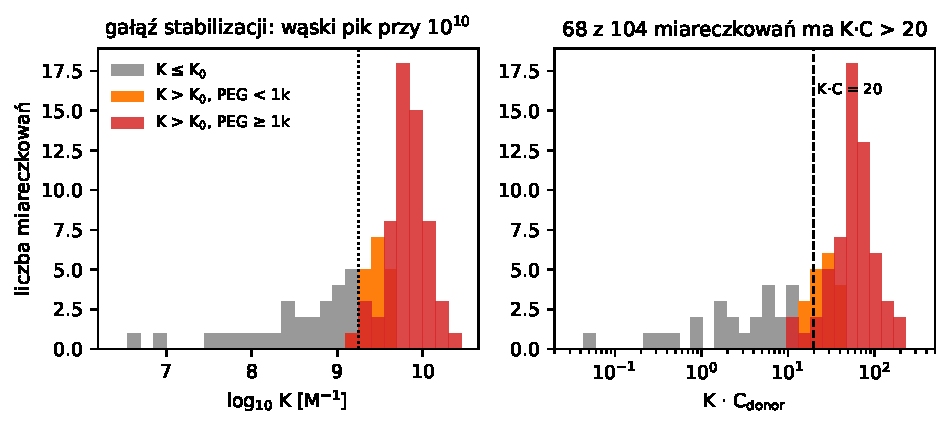
\includegraphics[width=0.95\linewidth]{figures/c1_distribution.pdf}
\caption{Rozkład dopasowanych $K$ i $K\cdot C_\mathrm{donor}$. Gałąź stabilizacji leży przy $K\cdot C\approx30$--$200$.}
\end{figure}

\section{Symulacja: gdzie zaczyna się sufit}
Dla każdego miareczkowania (te same stężenia akceptora, $\alpha$, $\gamma$, $V_0$ i $C$ ze skryptu, $D$ z dopasowania) wygenerowałem krzywe dla $K$ od $10^8$ do $10^{12}$ (co 0.25 dekady). Dodałem szum gaussowski o odchyleniu równym RMS reszt danego miareczkowania ($\CnRep$ powtórzeń, razem $\CnSim$ dopasowań) i dopasowałem je oryginalną funkcją (start $K=10^6$, te same granice). Dla PEG $\geq$1k odchylenie mediany i połówka przedziału 16--84\% w dekadach wynoszą: przy $10^9$: $\CsimMedNine$ / $\CsimWidNine$; przy $10^{10}$: $\CsimMedTen$ / $\CsimWidTen$; przy $10^{10.5}$: $\CsimMedTenHalf$ / $\CsimWidTenHalf$; przy $10^{11}$: $\CsimMedEleven$ / $\CsimWidEleven$. Mediana nie ma obciążenia, ale \textbf{rozrzut eksploduje między $10^{10.5}$ a $10^{11}$}. Sufit dla miareczkowania definiuję jako największe $K$, przy którym $|$bias$|<0.2$ i rozrzut $<0.3$~dex. Mediana dla PEG $\geq$1k wynosi $10^{\CceilMedLong}$ (zakres $10^{\CceilMinLong}$--$10^{\CceilMaxLong}$). Ponad własnym sufitem leży $\CnAboveCeil$ miareczkowanie.

\begin{figure}[h]
\centering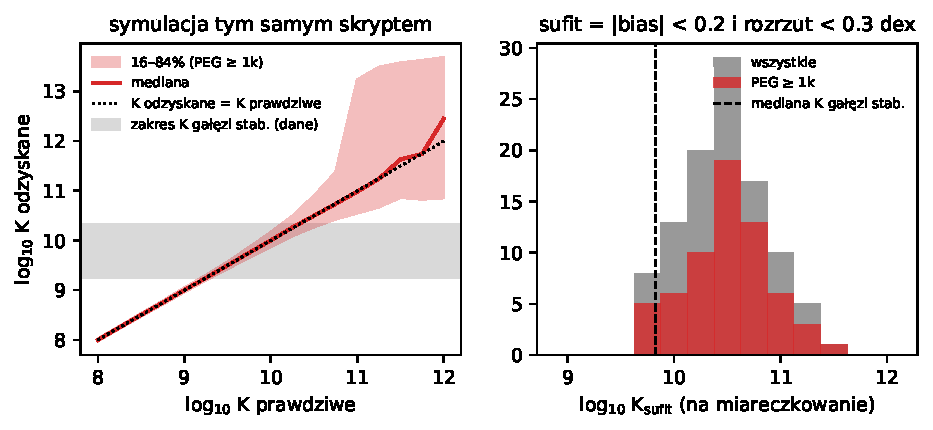
\includegraphics[width=0.95\linewidth]{figures/c2_simulation.pdf}
\caption{Odzyskane vs prawdziwe $K$ (szare pasmo: zakres danych gałęzi stabilizacji) i rozkład sufitów poszczególnych miareczkowań.}
\end{figure}

\section{Profile wiarygodności}
Dla siatki $K=10^5$--$10^{12}$ (141 punktów; zakres poszerzony w dół, bo EG przy 40\% ma $K<10^7$) minimalizowałem SSR po $D$ (te same granice co w skrypcie), z $V_0$, $\alpha$, $\gamma$ ustalonymi jak w skrypcie. $\Delta\chi^2=(\mathrm{SSR}(K)-\mathrm{SSR}_\mathrm{min})/(\mathrm{SSR}_\mathrm{min}/(n-2))$; przedział 95\%: $\Delta\chi^2\leq3.84$. Wariant odporny ma wolną amplitudę (wspólny czynnik $V_0\cdot$jasność, wyznaczany analitycznie), czyli $n-3$ stopnie swobody.
\begin{itemize}\itemsep1pt
\item $V_0$ ustalone: otwarta górna granica w $\CnUpUnb$ z $\CnAll$ przypadków; mediana szerokości przedziału 95\% to $\CwidthMed$~dex. Swobodne dopasowanie zawsze leży w globalnym minimum (rozbieżności: $\CnNotGlobal$).
\item Wolna amplituda: otwarta górna granica w $\CnUpUnbR$ przypadkach, wszystkie w gałęzi stabilizacji ($K\cdot C\geq\CKCminUnbR$), mediana szerokości $\CwidthRMed$~dex. Przesunięcie $K$ względem skryptu: mediana $\CshiftRMedAll$~dex, odchylenie $\CshiftRSD$~dex, skorelowane z V$_\mathrm{ef}$ ($\rho=\CrhoShiftVef$).
\end{itemize}

\begin{figure}[h]
\centering
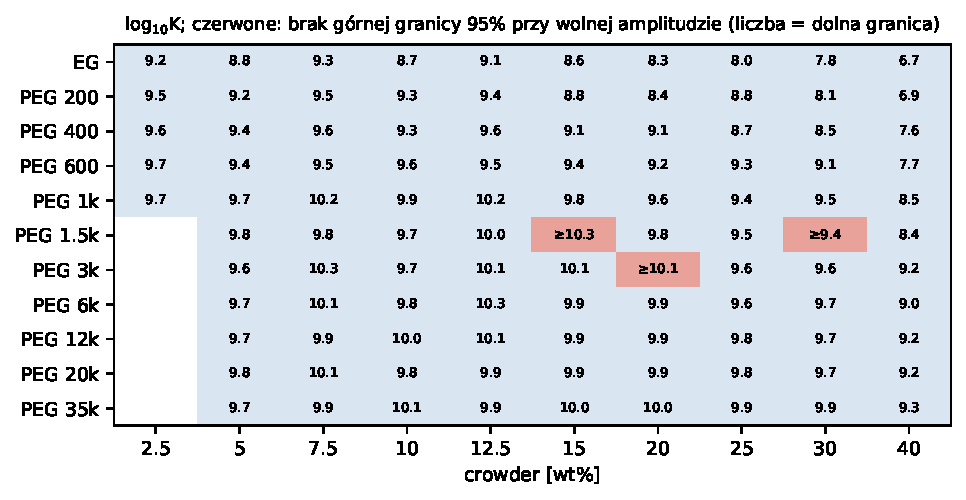
\includegraphics[width=0.62\linewidth]{figures/c3_profile_status.pdf}\hfill
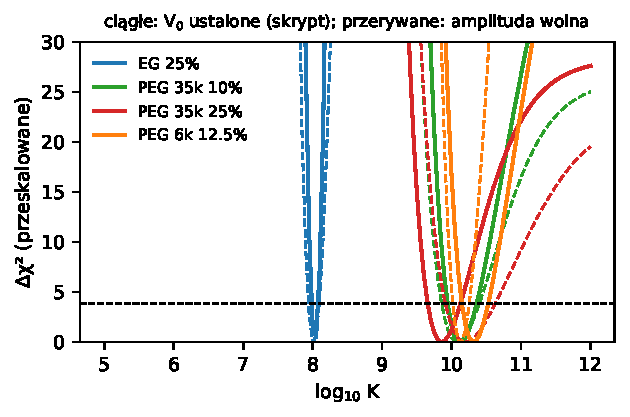
\includegraphics[width=0.36\linewidth]{figures/c3_profiles.pdf}
\caption{Lewo: status przedziału 95\% przy wolnej amplitudzie (czerwone: tylko dolna granica). Prawo: przykładowe profile.}
\end{figure}

\section{Analizy z raportu z cenzurowaniem}
Punkty bez górnej granicy (wariant odporny; $\CnCensPts$ punktów) traktuję jako cenzurowane: prawdziwe $\dG\leq$ wartość przy dolnej granicy 68\%, z wiarygodnością Tobita. Niepewności punktów biorę z profili (połowa przedziału 68\%), a dla punktów cenzurowanych z mediany danego crowdera.

\begin{center}
\begin{tabular}{lccc}
\toprule
wielkość & jak w raporcie & bez cenzurowanych & Tobit \\
\midrule
m/N, $N\geq13$, 0--5.5 monomolal [kcal/(mol·molal)] & $\CmNO\pm\CmNOErr$ & $\CmND\pm\CmNDErr$ & $\CmNT\pm\CmNTErr$ \\
$s_1$ przy $x^*=6$ & $\CsOneSixO\pm\CsOneSixOErr$ & $\CsOneSixD\pm\CsOneSixDErr$ & $\CsOneSixT\pm\CsOneSixTErr$ \\
$s_2$ przy $x^*=6$ & $\CsTwoSixO\pm\CsTwoSixOErr$ & $\CsTwoSixD\pm\CsTwoSixDErr$ & $\CsTwoSixT\pm\CsTwoSixTErr$ \\
$s_2$, $x^*$ swobodne & $\CsTwoFreeO\pm\CsTwoFreeOErr$ & $\CsTwoFreeD\pm\CsTwoFreeDErr$ & $\CsTwoFreeT\pm\CsTwoFreeTErr$ \\
$x^*$ swobodne (mediana; zakres) & $\CxsMedO$ ($\CxsLoO$; $\CxsHiO$) & $\CxsMedD$ ($\CxsLoD$; $\CxsHiD$) & $\CxsMedT$ ($\CxsLoT$; $\CxsHiT$) \\
$\Delta(-2\ln L)$: $x^*=6$ vs swobodne & $\CdChiSixFreeO$ & $\CdChiSixFreeD$ & $\CdChiSixFreeT$ \\
$x_\mathrm{min}$ PEG $\geq$1k (mediana; zakres) & $\CxminMedO$ ($\CxminLoO$--$\CxminHiO$) & $\CxminMedD$ ($\CxminLoD$--$\CxminHiD$) & $\CxminMedT$ ($\CxminLoT$--$\CxminHiT$) \\
\bottomrule
\end{tabular}
\end{center}
$\Delta G_\mathrm{rest}$ (PEG $\geq$3k, jak Fig.~4d): średnia $\CrestMeanAll$ (wszystkie), $\CrestMeanBounded$ (bez cenzurowanych, $\CrestFracCens$\% punktów cenzurowanych), odchylenie $\CrestSDBounded$~kJ/mol. \textbf{Cenzurowanie nie zmienia żadnego wniosku}; różnice między kolumnami wynikają z innego wyboru błędów punktów, a nie z cenzury.

\begin{figure}[h]
\centering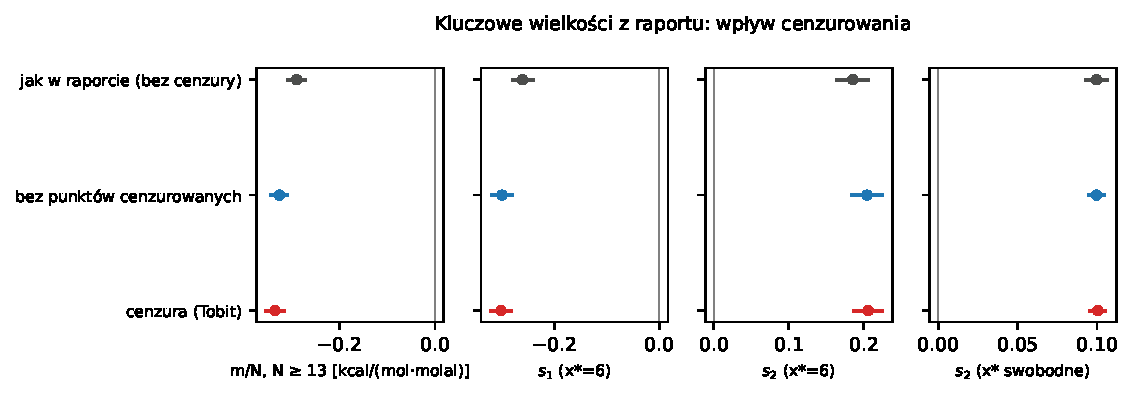
\includegraphics[width=0.95\linewidth]{figures/c4_censored.pdf}
\caption{Kluczowe wielkości przy trzech sposobach traktowania punktów.}
\end{figure}

\section{Kalibracja solna jako splajn}
Splajn kubiczny $\ln K(\ln c)$ (wagi $1/\sigma$, parametr wygładzenia $s=n$; bootstrap parametryczny, 2000 prób) daje SK$(c_0)=\CSKspline\pm\CSKsplineErr$ (16--84\%: $\CSKsplineLo$--$\CSKsplineHi$). Model $A+Be^{-k\sqrt c}$ daje $\CSKexp$, lokalne nachylenie z raportu $\CSKlocalReport$. Wariant (c) członu solnego przy 40~wt\% PEG 35k: $\CcFortySpl$ (splajn) vs $\CcFortyExp$~kJ/mol (model). Średni ułamek wahnięcia: (c) $\Cfraccspl\pm\CfraccsplUnc$\% vs $\Cfraccexp$\%; (e) $\Cfracespl$\% vs $\Cfraceexp$\%. \textbf{Wnioski tezy 2 nie zależą od formy kalibracji.} Splajn jest przy dziewięciu punktach falisty poniżej 10~mM, ale w okolicy $c_0$ i w przedziale $c_\mathrm{eq}$ (20--35~mM) jest stabilny.

\begin{figure}[h]
\centering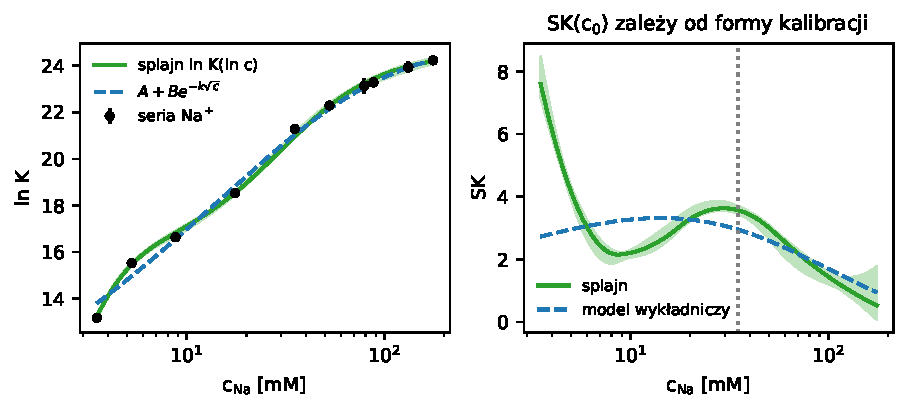
\includegraphics[width=0.85\linewidth]{figures/c5_spline.pdf}
\caption{Kalibracja solna: splajn z pasmem bootstrapu vs model wykładniczy; SK$(c)$.}
\end{figure}

\textbf{Założenia.} Szum homoskedastyczny w obrębie miareczkowania (RMS reszt); $D$ symulacji = $D$ z dopasowania; $\alpha$ i $\gamma$ traktowane jako dokładne (wariant odporny uwalnia tylko wspólną amplitudę, nie stosunek $\gamma/\alpha$); kalibracja solna tylko z \texttt{Na\_FRET.csv} ($\leq175$~mM).

\end{document}
